\documentclass{article}
\usepackage[russian]{babel} 
\usepackage{graphicx}
\graphicspath{{pictures/}}
\DeclareGraphicsExtensions{.pdf,.png,.jpg}
\title{Лабораторная работа №3}
\author{Тананов Алексей Александрович}
\date{2020}
\begin{document}
\maketitle
\newpage
\section{Описание предприятия}
\paragraph{ПО.}

Предприятие занимается техническим обслуживанием лифтового оборудования.

Программные продукты, используемые на предприятии: “Банк-клиент”, “1С-Бухгалтерия”, “Консультант-плюс”, “ГРАНД-Смета”, “Почтовый клиент”.

Администрация предприятия в лице директора имеет полный доступ к системам и данным. Бухгалтерия имеет доступ к “Банк-клиент” по ключу, “Почтовый клиент”, “1С-Бухгалтерия” и “Консультант-плюс”. Кадровый отдел имеет доступ к приложению “Консультант-плюс”, “Почтовый клиент”. Сметно-плановый отдел имеет доступ к приложению “Консультант-плюс”, “ГРАНД-Смета”, “Почтовый клиент”.  

Ниже приведено уравнение ~\ref{eq:solv}, необходимое по условию лабораторной работы.

\begin{equation}\label{eq:solv}
\int \limits_S \left( \frac{\partial Q}{\partial x} - \frac{\partial P}{\partial y} \right)\, dx \, dy =\oint \limits_C P\,dx + Q \, dy
\end{equation}
\newpage
\paragraph{Структура.}

Предприятие подразделяется на 5 отделов: администрация, отдел кадров, бухгалтерия, сметно-плановый отдел, рабочие бригады под руководством прорабов.

Офис включает в себя 3 кабинета. Кабинеты руководства и бухгалтерии расположены отдельно, сотрудники отдела кадров, сметно-планового отдела и рабочее место прорабов располагаются в общей рабочей зоне, размещенной по центру офиса. На рисунке ~\ref{fig:image} представлен план помещения.

Силовая сеть в исправном состоянии, розетки 220 В имеются в количестве 3 штук возле каждого рабочего места и дополнительно под офисное оборудование (принтер) в точке “B” на плане офиса, серверное оборудование в точке “A” на плане офиса.

\begin{figure}[h]
	\center{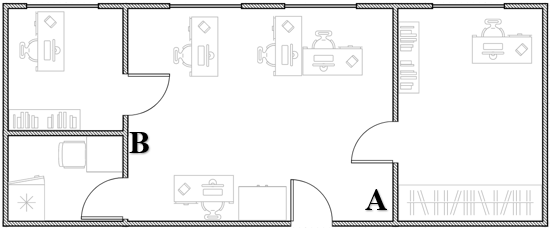
\includegraphics[scale=0.65]{image}}
	\caption{План офиса}
	\label{fig:image}
\end{figure}
\newpage
\tableofcontents
\end{document}